\documentclass[10pt,twocolumn]{article}
\usepackage[english]{babel}
\usepackage{amssymb}
\usepackage{amsmath}
\usepackage[left=1.5cm, right=1.5cm]{geometry}
\usepackage{csquotes}
\usepackage{caption}
\usepackage{graphicx}
\usepackage{multicol}
\usepackage{listings}
\usepackage{minted}
\usepackage[dvipsnames]{xcolor}
\usepackage[backend=biber,sorting=none]{biblatex}
\addbibresource{references.bib}
% \graphicspath{ {./images/} }
\setminted[python]{breaklines}

\begin{document}

\title{Computational Neuroscience: \\ Inhibitory-Stabilised Networks}
\author{B204511}
\date{November 2024}
\maketitle

\section{Introduction}
Several brain regions, including the neocortex and hippocampus \cite{tsodyks1997paradoxical}
contain local recurrently connected networks of excitatory and inhibitory neurons.
Understanding how those networks function and react to external inputs is important
for analysing how the brain operates. This report will introduce the concept of
such networks, discuss their biological relevance, present a mathematical model, and provide
computer simulations as well as mathematical analysis of the model.

The network is viewed as consisting of 2 pools of neurons: excitatory and inhibitory.
Each pool projects to the other, and to itself, forming a recurrent neural network.
Excitatory feedback can lead to runaway excitation, which is prevented by the inhibitory feedback.
This allows the network to stabilise, earning it the name Inhibitory-Stabilised Network (ISN).


To understand how the system comes together, it is important to get a sense of what
the underlying model of each individual nueron is and how the interaction between them integrates.

% #######################
% Model of the Neuron
% #######################

\subsection{Leaky Integrate-and-Fire Neuron}
In 1907, Louis Édouard Lapicque \cite{brunel2007quantitative} introduced
the concept of the integrate-and-fire neuron model.
Even though the model was developed before scientists
had a chance to describe the biophysical mechanics of the neuron,
it captured the behaviour of the neuron in a way that was useful
for understanding \cite{abbott1999lapicque}.

The neuron is viewed as an electric circuit with a capacitor and a resistor connected in parallel.
% resistor
The membrane has some resistance, which is assumed to be constant and can be described by Ohm's law: $V = IR$, and therefore
the resistor current is $I = \frac{V}{R} = gV$, where $g$ is conductance of the cell.
% capacitor
The relationship between the current and the voltage across the capacitor is described by the following equation:
$C = \frac{Q}{V}$, where $C$ is the capacitance, $Q$ is the charge stored in the capacitor, and $V$ is the voltage across the capacitor.
Knowing this, the current in the circuit:

$$
    I = \frac{dQ}{dt} = \frac{dCV}{dt} = C \frac{dV}{dt}
$$
% Combining the two, we get: $C \frac{dV}{dt} = gV$.

Real neurons, however, receive current from other neurons via dendrites from synapses,
and induce own \textbf{ionic} current by
% opening and closing ion channels (each with its own conductance) and 
letting charged particles
% ($Na^+, Cl^-, Ca^{2+}, K^+$) 
in and out of the cell. Therefore,
the total current is the sum of the ionic current plus any external input: $I = \sum_{i}g_iV + I_{ext} = g_mV + I_{ext}$.
Neurons are generally \textbf{negatively charged} relative to the outside, and therefore the flow outside the cell is treated as positive.
Since the size of the cell and its channels is comparable to that of ions, effect of electric attraction is comparable with that of diffusion,
and there exists a point, where one balances out the other, resulting in the zero net current flow.
This point is called the resting potential $V_{rest}$ of the neuron, and therefore any current should be measured relative to this potential.

$$
    C \frac{dV}{dt} = -g_m(V - V_{\text{rest}}) + I_{\text{ext}}
$$

Dividing by conductance, we get the following equation:
$$
    \tau_m \frac{dV}{dt} = -(V - V_{\text{rest}}) + \frac{I_{\text{ext}}}{g_m}
$$
where $\tau_m$ is the membrane time constant, describing how quickly it reacts to input.

Now, the external current is the component of interest,
by extending this component, we can integrate input from other neurons.
Neurons communicate by sending electrical signals to each other, via the synapse of
emitting through the dendrites of the receiving neuron.
This interaction can be modelled as a synpatic current, weighted by the strength of connection.
Dale's Law\cite{efron1968psychopharmacology} states that a neuron can only be
either excitatory or inhibitory, and therefore we can simplify the model, and
approximate the synaptic current as a function of emitting neuron's voltage:
$I_{\text{syn},i} = W\phi(V_i)$,
where $W$ is the synaptic weight ($+$ for excitatory, $-$ for inhibitory), and $\phi(V)$ is the transfer function of the neuron.
The actual external current collapses into $I_{ext}/g_m=u_{ext}$.

Combing all component, we obtain a system of equations:
\begin{equation}
    \tau_E \frac{dV_E}{dt} =
    -(V_E - V_{\text{rest}})
    + W_{EE} \phi(V_E)
    - W_{EI} \phi(V_I) + u_E
\end{equation}

\begin{equation}
    \tau_I \frac{dV_I}{dt} =
    -(V_I - V_{\text{rest}})
    + W_{IE} \phi(V_E)
    - W_{II} \phi(V_I) + u_I
\end{equation}
where $V_{\text{rest}}$ is the resting potential of the neuron, $W_{k}$ are the
synaptic weights, $u_k$ are the external inputs to neurons,
and $\phi(V)$ is the transfer function of a neuron, that acts as
a communication channel between the neurons and is defined as a scaled ReLU function:

\begin{equation}
    \phi(V) = \beta[V-V_0]_+
\end{equation}

Now that we have the model and its origins, it's important to outline
the benefits and limitations of the model.

\subsection{Considerations (Q1)}
1. The model abstracts away certain biological complexity, such as stochasticity and
variability of individual ion channels (both in somas and synapses), described in
great detail by the Hodgkin-Huxley model \cite{hodgkin1952quantitative}, which is
a more biologically plausible model of the neuron,
but is also signficantly more complex.

2. Synaptic weights are a heuristic approximation of synpatic conductances
and assumed to be constant, whereas in reality they are
subject to plasticity, and can change over time.

3. The input activity from the opposite neural pool is treated as a
linear function of its voltage with an activation threshold,
which is not realistic as neurons spiking activity varies depending
on its structure and intrinsic properties \cite{izhikevich2003simple}.

3. The membrane time constant that comes from conductance is assumed
to be constant, and its usage relies on Ohm's law holding, which is
a simplification of the actual behaviour of a neuron.
However, it is a good approximation for the passive dynamics of a neuron
which makes the model tractable for analysis.

4. The LIF model is a lot more computationally affordable, requires 4 ODEs
per neuron in the HH model, instead of 1 in the LIF model,
which allows us to run large scale simulations and analyse
the network behaviour faster. The model is also more amenable
to theoretic analysis, which helps to explain certain activity patterns in the network.

In essence, we trade off biological accuracy for
computational efficiency and analytic tractability.


% ####################### 
% COMPUTER SIMULATIONS
% #######################

\section{Computer Simulations}
In this section, simulations of the network are presented,
where the network is stimulated with various external inputs for
both excitatory and inhibitory pools, and the
response of the network is approximated numerically using the Euler method.
Python code used for simulations can be found in Appendix A.

In our simulations, we study 2 networks with the following base parameters:
% V_rest
$$
    V_{\text{rest}} = -70 \text{mV, } V_0 = -55 \text{mV, } \beta = 1
$$

% tau
$$
    \tau
    = \begin{pmatrix} \tau_E \\ \tau_I \end{pmatrix}
    = \begin{pmatrix} 20 \\ 10 \end{pmatrix}\text{ms}
$$

% Us
$$
    u
    = \begin{pmatrix} u_E \\ u_I \end{pmatrix}
    = \begin{pmatrix} 20 \\ 20 \end{pmatrix}
$$

% Ws
$$
    W
    = \begin{pmatrix} W_{EE} & W_{EI} \\ W_{IE} & W_{II} \end{pmatrix}
    = \begin{pmatrix} W^n_{EE} & 0.65 \\ 1.2 & 0.5 \end{pmatrix}
$$

where $W^n_{EE}$ is the weight of the excitatory feedback for a given network.
The 2 networks differ in the weight of the excitatory feedback, where one is weaker
is $W^1_{EE} = 0.5$ and the other is stronger $W^2_{EE} = 1.25$.

\begin{figure*}
    \centering
    \captionsetup{justification=centering}
    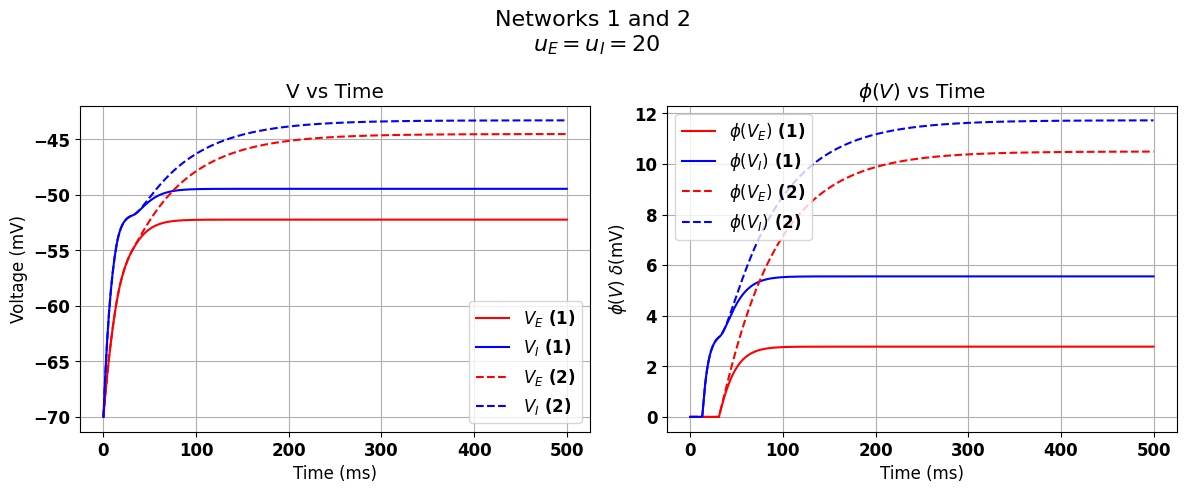
\includegraphics[width=1\textwidth]{images/12-stable.png}
    \caption{
        \textbf{Stable} external input to both neurons.\hspace{\textwidth}
        \textcolor{red}{Excitatory} potentials are red, \textcolor{blue}{Inhibitory} potentials are blue.\hspace{\textwidth}
        Network 1 is solid, Network 2 is dashed.
    }
    \label{fig:stable-input}
\end{figure*}

\subsection{Stable External Input (Q2)}
We first study both networks subjected to a stable external input of 20mV to
both neurons.
Both neurons start from the resting potential. The simulation is ran for 500ms
with 1ms time steps. The results are shown in Figure \ref{fig:stable-input}.

Looking at the results for Network 1 (solid lines), we can see that both neurons
gradually begin responding to the external input. Since $\tau_I < \tau_E$,
one might expect the \textcolor{blue}{inhibitory} neuron to respond faster, which is
exactly what is observed. The transfer function $\phi(V)$ is not immediately
responding to the increase in voltage as both neurons have to reach the threshold
potential, which matches with the timeline of both neurons reaching $V_0=-55mV$
and begin firing to provide input to the other. After about $5\tau$, as
expected with a capacitor behaviour, the system reaches a stable state
and both neurons' activity plateaus. At this point, $V_I$, however,
is about 3mV above $V_E$, which could be due to a stronger $W_{IE}$ connection
relative to $W_{EI}$, given that the feedback strength to both neurons is equal,
excitation of I is stronger than inhibition of E, and therefore less $V_E$
is needed to balance out $V_I$.

\subsection{Inhibitory Input Increase (Q3-4)}
\begin{figure*}
    \centering
    \captionsetup{justification=centering}
    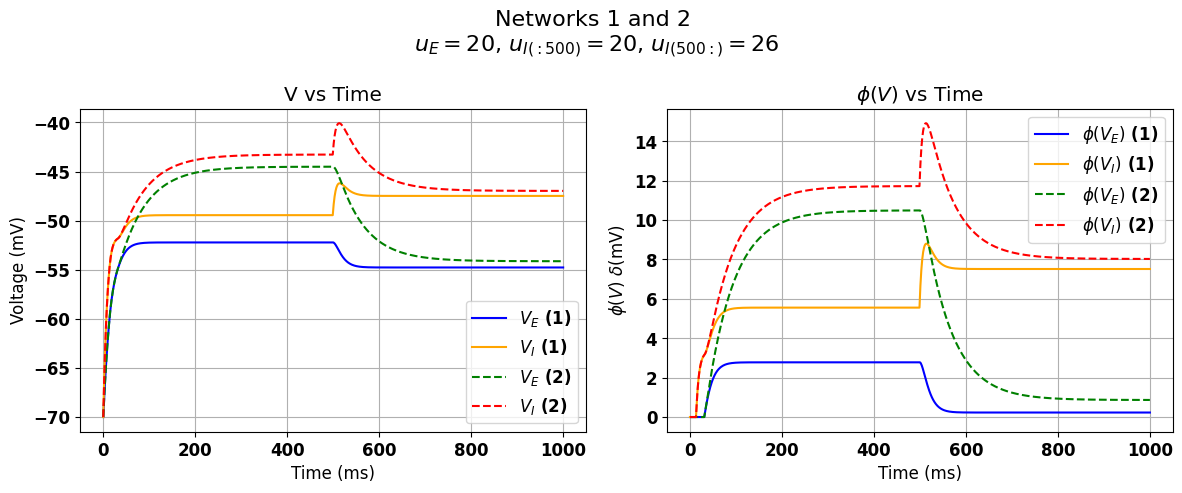
\includegraphics[width=1\textwidth]{images/12-I_input.png}
    \caption{External \textbf{inhibitory} input increase after 500ms.\hspace{\textwidth}
        \textcolor{red}{Excitatory} potentials are red, \textcolor{blue}{Inhibitory} potentials are blue.\hspace{\textwidth}
        Network 1 is solid, Network 2 is dashed.}
    \label{fig:i-input}
\end{figure*}

Both networks are simulated for further 500ms with
an increase in $u_I$ from $20$mV to $26$mV. The results for
this simulation are shown in Figure \ref{fig:i-input}.

Network 1, prior to the $u_I$ increase, is in a stable state, and immediately after
inhibitory activity naturally increases. As $V_I$ increases, according to
eqaution (1), $V_E$ decreases, which is expected. 10ms later, inhibitory activity
peaks and then drops slightly to stabilise once again, the peak and drop can be
explained by equation (2), that tells us that $V_I$ depends on weighted ReLU'd
activity of $V_E$, which has been decreasing previously and therefore at some point
decreasing excitatory activity will begin balancing out external inhibitory input
and we'd expect the network to begin approaching a stable state. Stable state
is eventually reached at about 570ms, where potentials settle once again, however,
$V_I$ is above its previous stable value, and $V_E$ is below. This makes sense
following the logic from the stable external input simulation - stronger $W_{IE}$
connection tells us that less excitatory activity is needed to
balance out the inhibitory.

For Network 2 (dashed lines), the results are similar but with a subtle difference. Both pools
are responding to the input as described above: inhibitory spike, then excitatory dip,
followed by the dip in inhibitory activity and eventual stabilisation. However,
this time round, the final stable state is below the original for both neurons,
which seems counterintuitive as the increase in inhibitory activity leads
to a reduction in the activity of the whole network. The paradox here would
be that, for some reason, the activity is not balancing like in Network 1,
but decreases overall. Since the only parameter that differs is the
$W_{EE}$ synaptic weight, the behaviour can attributed to it.

\subsection{Excitatory Input Increase (Q5)}
We will now simulate an increase in external Excitatory input, unlike Inhibitory
in the previous section. Similarly, both neurons are reaching a stable state
with constant 20mV input to both, when a similar increase to 26mV in $u_E$ occurs.
The results can be observed in Figure \ref{fig:e-input-unclamped}

As before, prior to the change, the system is in a stable state. When the
excitatory neuron's external stimulation increases, unsurprising increase
in excitatory activity follows, causing the inhibitory activity to rise
    [Equation (2)], which inhibits the excitatory neuron itself, flattening
the rate of change and eventually stabilising the system.
All of the observations are intuitive and follow from the equations
describing the system. Both networks behave similraly, but of course,
with a subtle difference - before the increase, stable state of
both networks has the inhibitory potential above excitatory,
in Network 1 that is still the case after the system adapts to the
change, however in Network 2, the excitatory stable potential now
exceeds that of the inhibitory.

\begin{figure*}
    \centering
    \captionsetup{justification=centering}
    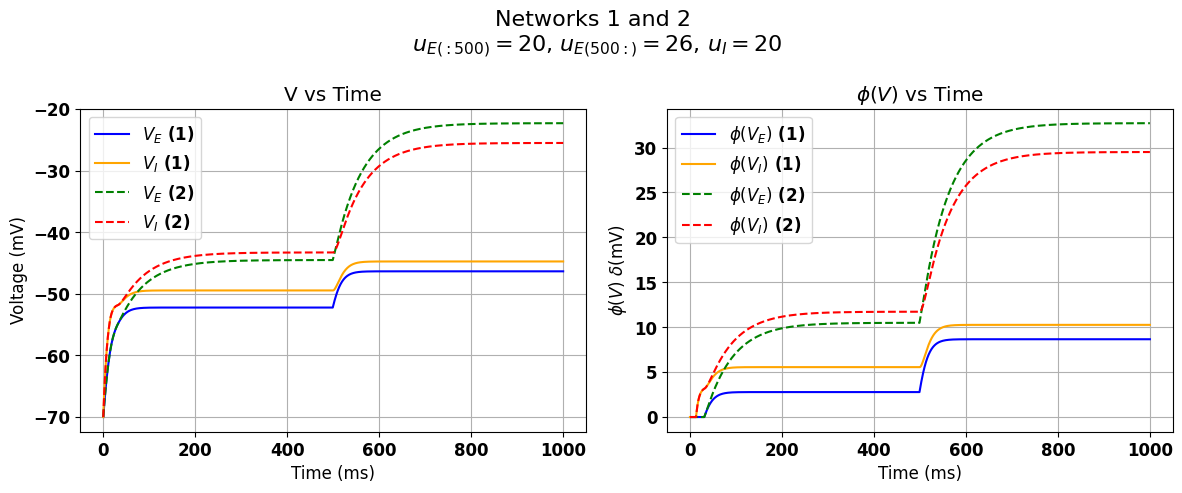
\includegraphics[width=1\textwidth]{images/12-E_input.png}
    \caption{External \textbf{excitatory} input increase after 500ms. $V_I$ unclapmed \hspace{\textwidth}
        \textcolor{red}{Excitatory} potentials are red, \textcolor{blue}{Inhibitory} potentials are blue.\hspace{\textwidth}
        Network 1 is solid, Network 2 is dashed.}
    \label{fig:e-input-unclamped}
\end{figure*}

Stronger excitatory feedback combined with a relatively higher external
stimulation push the neuron towards an endless excitation, so the
inhibitory neuron by extension begins gauging the runaway activity,
thus stabilising the network. This behaviour can once again be
attributed to a different weight of the synaptic Excitatory feedback.

This experiment kept the network in tact, while stimulating the
excitatory neuron and in both cases the system returned to a
stable state. There is a very short delay before the inhibitory
neuron begins catching up, which according to the Equation 1 and
the observations confirms to us that the inhibitory neuron prevents
the runaway excitation of E.

In this next experiment, we will stimulate
the excitatory neuron once again, but this time clamp the inhibitory
neuron for it to remain at the resting potential. The results of this
simulation are show in Figure \ref{fig:e-input-clamped}.
With the inhibitory neuron clamped, the excitatory neuron is free to
excite indefinitely, however, in network 1, the activity eventually stabilises
as the inhibitory neuron still provides feedback to the excitatory neuron.
In network 2, on the other hand, the excitatory feedback is much stronger
relative to the inhibitory, and the E neuron continues increasing activity
indefinitely. To spare the scale of indefinite (bilogoically unrealistic) 
simulation, I have limited the max voltage displayed on the graph, but it is
clear that the activity explodes in the first 100ms, even before the 
external input is increased.

\begin{figure*}
    \centering
    \captionsetup{justification=centering}
    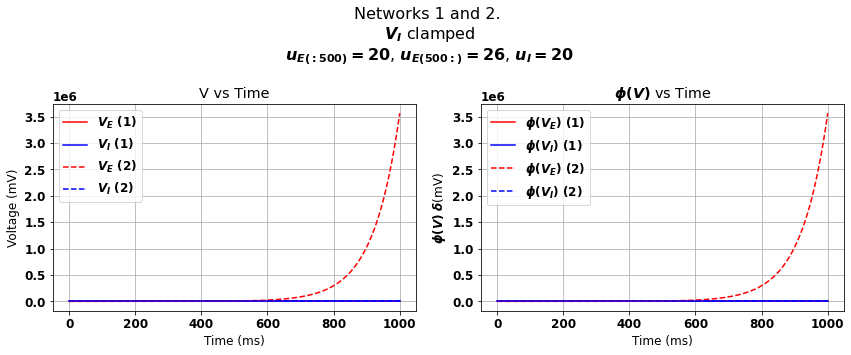
\includegraphics[width=1\textwidth]{images/12-E_input_V_I_clamped.png}
    \caption{External \textbf{excitatory} input increase after 500ms. $V_I$ clapmed \hspace{\textwidth}
        \textcolor{red}{Excitatory} potentials are red, \textcolor{blue}{Inhibitory} potentials are blue.\hspace{\textwidth}
        Network 1 is solid, Network 2 is dashed.}
    \label{fig:e-input-clamped}
\end{figure*}

\subsection{Stabilisation and Paradoxical Inhibition (Q6)}
To sum up findings so far: a network is called ISN if the Excitatory component is unstable
alone, but combined with the inhibitory it is.
The purpose of ISN is to prevent runaway excitation and
maintain the balance in a neural network. Paradoxical inhibition is
a counterintuitive reaction of a network, where external inhibitory input
causes the overall activity of the network to decrease.
Both are most certainly related to the external input, the synaptic weights
and the intrinsic properties of each neuron. 

Based on the simulations, it looks like it is more
affected by the synaptic weights between neurons (including feedback)
 when the system is adapting to the input to reach a stable state. 
In particular, on the excitatory feedback strength relative to the 
inhibitory feedback strength.

Based on the above, it seems reasonable to suppose that 
low $W_{EE}$ to $W_{II}$ ratio ($\le1$)  keeps the network stable and 
high ($>1$) leads to an unstable behaviour, including paradoxical 
inhibition and runaway excitation.

\subsection{Discussion (Q7-8)}
The simulations above gave us a glimpse of what the network response
is like under different conditions to variying external inputs.
However, the simulations are limited in that they only show what 
it looks like given the input we have manually set, and therefore
do not provide a comprehensive understanding of the network behaviour.
Given that the model has $2\times 6=12$ parameters for 2 neurons,
and each can be varied to influence the behaviour.
%  
And while the first 10 of them are describing the neurons, 
the other 2 do external inputs, which can vary in time and shape and 
running simulations on a specific pattern of external input might not 
definitively explain the relationship in general.
One alternative way to analyse the model to gain more insight 
into how inhibitory stabilisation relates to the paradoxical inhibition, 
we might look at a more theoretic approach, including 
mathematical analysis of the system. 
% 
Another way would be to try and limit the scope of the problem
by limiting parameters we're simulating for based on the biological data.
Those can be estimated from data gathered in vitro or in vivo, 
we could study the brain further to understand what the sources
of external input are, and how they vary in time and space,
Tsodyks highlights \cite{tsodyks1997paradoxical} that there are 
Theta and Gamma oscillations in the brain, which are common
sources of external input to the network.
% 
Since the model is based on several big assumptions, how can we be sure
that the networks in brain are in fact operating in the ISN regime?
One way to test this would be to record the activity of the neurons
and observe the activity (using EEG or fMRI) given different
stimuli. This is an overly simplistic approach, and the brain has
many components, each with its own dynamics and local networks,
all of which together interfere with the activity of the network,
and it's hard to isolate the isolate both the network activity
and the inputs to it.
Another way would be to use a novel optogenetics approach
to embed light-sensitive channels into neural membrane and 
manipulate the activity with light. This approach allows for high 
precision and control over the activity of the neurons, but 
is limited to animal models and is not yet ready for 
human use \cite{sadeh2021inhibitory}.
%  

\section{Mathematical Analysis}
In this section, we will provide a mathematical analysis
of the network model and explore the relationship between
the inhibitory stabilisation and paradoxical inhibition.

Assuming, $V > V_0$, we can drop the non-lineraity of the activation
function and expand the expression to do some algebra.

\subsection{Reformulation (Q9)}
To simplify the analysis, we can reformulate the system
of equations describing the network and
express it in the matrix-vector form:

$$
    \frac{d\textbf{V}}{dt}
    = A\textbf{V} + \textbf{x}
    =
    \begin{pmatrix}
        A_{EE} & A_{EI} \\
        A_{IE} & A_{II}
    \end{pmatrix}
    \cdot \begin{pmatrix} \textbf{V}_E \\ \textbf{V}_I \end{pmatrix}
    + \begin{pmatrix} \textbf{x}_E \\ \textbf{x}_I \end{pmatrix}
$$

where $A$ is the matrix of synaptic weights,
and $\textbf{x}$ is the external input.
To find the values of each term, Vs are factored out, and
constant terms are grouped together based on equations (1) and (2).
% grouping terms
$$
    \begin{align*}
        \frac{d\textbf{V}_E}{dt} & = \textbf{V}_E \boxed{\frac{-1 + W_{EE}\beta}{\tau_E}}
        + \textbf{V}_I \boxed{\frac{-W_{EI}\beta}{\tau_E}}                                           \\
                                 & + \boxed{\frac{V_{rest} + V_0\beta(W_{EI}-W_{EE}) + u_E}{\tau_E}}
    \end{align*}
$$

$$
    \begin{align*}
        \frac{d\textbf{V}_I}{dt} & = \textbf{V}_E\boxed{\frac{W_{IE}\beta}{\tau_I}}
        + \textbf{V}_I\boxed{\frac{-1 - W_{II}\beta}{\tau_I}}                                        \\
                                 & + \boxed{\frac{V_{rest} + V_0\beta(W_{II}-W_{IE}) + u_I}{\tau_I}}
    \end{align*}
$$

Now the system can be rewritten in the matrix form:
$$
    \begin{gathered}
        \frac{d\textbf{V}}{dt}
        =
        \begin{pmatrix}
            \frac{-1 + w_{EE}\beta}{\tau_E} & \frac{-w_{EI}\beta}{\tau_E}     \\
            \frac{w_{IE}\beta}{\tau_I}      & \frac{-1 - w_{II}\beta}{\tau_I}
        \end{pmatrix}
        \begin{pmatrix}
            \textbf{V}_E \\ \textbf{V}_I
        \end{pmatrix}+
        \\
        +
        \begin{pmatrix}
            \frac{V_{rest} + V_0\beta(W_{EI}-W_{EE}) + u_E}{\tau_E} \\
            \frac{V_{rest} + V_0\beta(W_{II}-W_{IE}) + u_I}{\tau_I}
        \end{pmatrix}
    \end{gathered}
$$


\subsection{Steady State (Q10-11)}
The steady state of the system $\textbf{V}^\ast_E,\textbf{V}^\ast_I$ is defined  by
both derivatives being zero. Since $\tau$ are non-zero constant terms, we can drop
them from the equation, and solve for the steady state:

$$
    \begin{pmatrix}
        0 \\ 0
    \end{pmatrix}
    =
    \begin{pmatrix}
        A_{EE} & A_{EI} \\
        A_{IE} & A_{II}
    \end{pmatrix}
    \begin{pmatrix}
        \textbf{V}^\ast_E \\ \textbf{V}^\ast_I
    \end{pmatrix}+
    \begin{pmatrix}
        \textbf{x}_E \\ \textbf{x}_I
    \end{pmatrix}
$$

Rearranging the terms, the solution for steady state voltages:

$$
    \begin{align*}
        \begin{pmatrix}
            \textbf{V}^\ast_E \\ \textbf{V}^\ast_I
        \end{pmatrix}
         & =
        -\begin{pmatrix}
             A_{EE} & A_{EI} \\
             A_{IE} & A_{II}
         \end{pmatrix}^{-1}
        \begin{pmatrix}
            \textbf{x}_E \\ \textbf{x}_I
        \end{pmatrix} \\
         & =
        \frac{-1}{det(A)}
        \begin{pmatrix}
            A_{II}  & -A_{EI} \\
            -A_{IE} & A_{EE}
        \end{pmatrix}
        \begin{pmatrix}
            \textbf{x}_E \\ \textbf{x}_I
        \end{pmatrix}
    \end{align*}
$$
To compute the determinant:
$$
    \begin{gathered}
        \textbf{det(A)} = A_{EE}A_{II} - A_{EI}A_{IE} \\
        = (W_{EE}\beta-1)(-W_{II}\beta-1) - W_{EI}\beta (-W_{IE}\beta)\\
        = \boxed{\beta^2(W_{IE}W_{EI}-W_{EE}W_{II}) + \beta(W_{II}+W_{EE}) + 1}
    \end{gathered}
$$

From the solution, we can derive the expression for
inhibitory steady state voltage $\textbf{V}^\ast_I$ in terms of network parameters:

$$
    \begin{gathered}
        \textbf{V}^\ast_I
        = \frac{-(- A_{IE}\textbf{x}_E + A_{EE}\textbf{x}_I)}{det(A)}
        = \frac{A_{IE}\textbf{x}_E - A_{EE}\textbf{x}_I}{det(A)}\\
        = \boxed{\frac{W_{IE}\beta \textbf{x}_E - (W_{EE}\beta - 1) \textbf{x}_I}{det(A)}}
    \end{gathered}
$$

To try and understand why the paradoxical inhibition occurs, we can study
what happens to the stable state inhibitory voltage when the external
inhibitory input is changing. To do so, we can differentiate $\textbf{V}^\ast_I$
with respect to $\textbf{u}_I$:

$$
    \begin{gathered}
        \frac{d\textbf{V}^\ast_I}{d\textbf{u}_I}
        = \frac{d}{du_I}\left(\frac{W_{IE}\beta \textbf{x}_E - (W_{EE}\beta - 1) \textbf{x}_I}{det(A)}\right)\\
        = \frac{W_{IE}\beta}{det(A)}\times\frac{d\textbf{x}_E}{d\textbf{u}_I} 
        - \frac{W_{EE}\beta - 1}{det(A)}\times\frac{d\textbf{x}_I}{d\textbf{u}_I}\\
        %
        = \frac{W_{IE}\beta}{det(A)}\times 0 
        - \frac{W_{EE}\beta - 1}{det(A)}\times 1\\ 
        = \boxed{\frac{-W_{EE}\beta + 1}{det(A)}}
    \end{gathered}
$$

To spare the complexity of the full expansion, both expressions keep 
$\textbf{x}_E$ and $\textbf{x}_I$ as variables, but they can be 
substituted with the actual values of the external input
derived above. The complete derivations can be found in the Appendix.

In the simulations, we observed that the both neurons' steady state
voltage (plateau value) decreased when the external inhibitory input $\textbf{u}_I$ increased.
To understand why this is happening, we can look at the conditions
under which this occurs. That is, when the derivative with respect to
external inhibitory input is negative:

$$
    \frac{d\textbf{V}^\ast_I}{d\textbf{u}_I}=\frac{-W_{EE}\beta + 1}{det(A)} < 0
$$

This gives us 2 cases to consider:
$$
    \begin{cases}
        -W_{EE}\beta + 1 > 0 & \text{if } det(A) < 0 \\
        -W_{EE}\beta + 1 < 0 & \text{if } det(A) > 0
    \end{cases}
$$
The 2 cases give us the exact conditions under which the paradoxical inhibition occurs.

\section{Discussion (Q12)}
In the simulations, we observed the behaviour of the 2 networks,
reacting to changes in external output and concluded that 
paradoxical inhibition had something to do with external input
and the weight of the synaptic excitatory feedback. 
To recap, the networks had the following weights: $W^1_{EE} = 0.5$ and $W^2_{EE} = 1.25$.
And it was Network 2 that exhibited the paradoxical inhibition.
Now that we have a mathematical explanation of this behaviour, let us 
compare the findings. Assuming that the system is not stable when $det(A) < 0$, 
the first inequality case can be ignored. The second case tells us that
the paradoxical inhibition occurs when $-W_{EE}\beta + 1 < 0$,
or when $W_{EE} > \frac{1}{\beta}$. Provided that $\beta = 1$, so
the condition becomes $\textbf{W}_{EE} > \textbf{1}$.
Clearly, Network 2 satisfies the condition and the puzzle is solved.

As mentioned before, the purpose of the ISN is to maintain the balance
and prevent endless excitation, while paradoxical inhibition is the overall
decrease in network activity due to increased input. Since the parameter 
of interest here is Excitatory feedback weight, the relationship could
be generalised to being a kill switch when the excitatory activity
becomes too high and inhibits the network accordingly.

\section{Paradoxical Excitation (Q13)}
To hypothesize, whether a analogus process - Paradoxical Excitation - could take place,
we can define this similarly to Paradoxical Inhibition. That would mean
the overall network activity decreases as external excitatory input $u_E$
increases. Similarly, we can look at the derivative of the stable state 
voltage $\textbf{V}^\ast_E$ with respect to $u_E$:
$$
    \begin{gathered}
        \frac{d\textbf{V}^\ast_E}{d\textbf{u}_E}
        = \frac{d}{du_E}\left(-\frac{(-W_{II}\beta-1) \textbf{x}_E + W_{EI}\beta \textbf{x}_I}{det(A)}\right)\\
        = \frac{W_{II}\beta+1}{det(A)}\times 1 
        - \frac{W_{EI}\beta}{det(A)}\times 0\\
        = \boxed{\frac{W_{II}\beta+1}{det(A)}}
    \end{gathered}
$$
Following the same logic as before, the paradoxical excitation occurs
when the derivative is negative, or when $W_{II}\beta + 1 < 0$.
This gives us the condition under which the paradoxical excitation occurs.
Skipping the negative determinant case, we can conclude that for the
paradoxical excitation to occur, the condition is $W_{II}\beta < -1$.
It is unclear how to interpret negative weights, as technically
that violates the Dale's Law, since our model accounts for inhibitory
input as negative, and therefore making it act as excitatory. 
So the paradoxical excitation might is not possible in this model.

\section{Conclusion}
To conclude, we have introduced the concept of Inhibitory-Stabilised Networks,
derived the model, simulated the network and analysed it mathematically, to investigate
 the dynamics of a neural network with 2 pools of neurons.

The model, based on a leaky integrate-and-fire, captures the essential 
interactions within neural circuits, in which the excitatory feedback can lead to 
runaway activity, but inhibitory feedback counters this, stabilizing the network. 
Over the simulations, the behavior of networks with differing excitatory feedback strengths was 
examined under varying external inputs, demonstrating the roles of synaptic weights and external 
stimulation in modulating network activity.

The simulations showed that networks with weaker excitatory feedback (Network 1) stabilize 
effectively in response to increased external input, exemplifying typical inhibitory-stabilized 
network behavior. In contrast, networks with stronger excitatory feedback (Network 2) 
exhibit paradoxical inhibition, where increased inhibitory input paradoxically results 
in an overall reduction of network activity. Mathematical analysis supports these observations, 
providing more concrete explanation for how synaptic weights, and in particular the 
excitatory feedback strength, influence the stability 
and paradoxical responses of the network. 


\clearpage
\printbibliography

\clearpage
\appendix
\section{Derivation of $\textbf{V}^\ast_I$ and $\frac{\textbf{V}^\ast_I}{d\textbf{u}_I}$}
% \noindent
\begin{figure}[ht]
    \centering
    \captionsetup{justification=centering}
    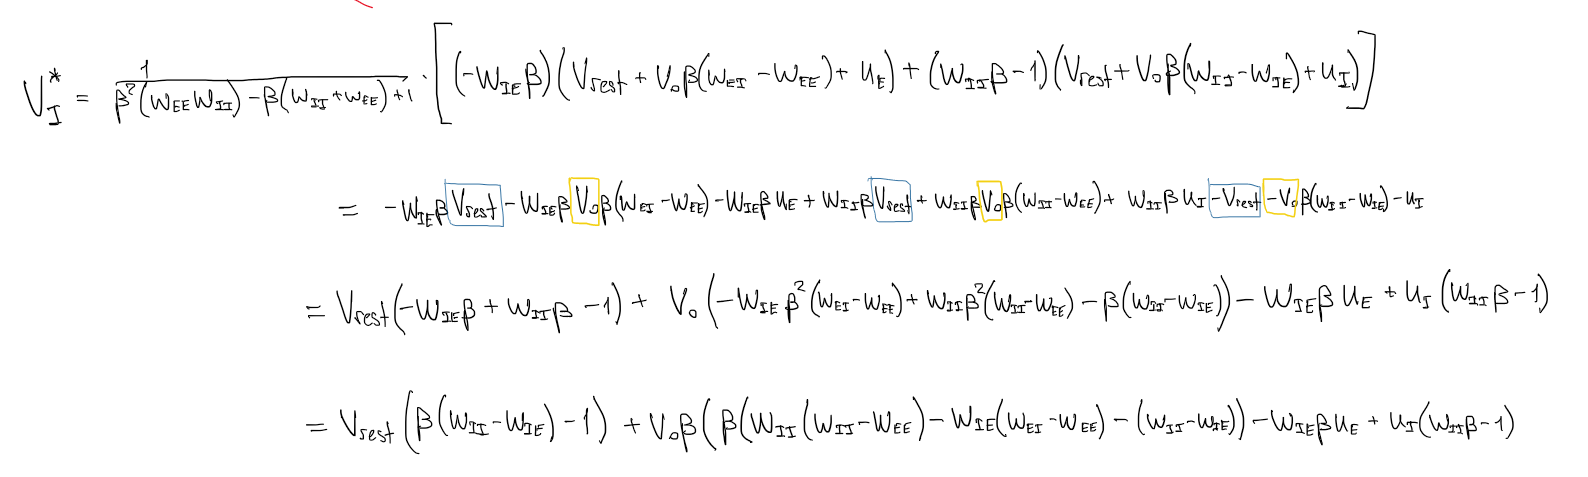
\includegraphics[width=1\textwidth]{images/Vi_derivation.png}
    \label{fig:vi-derivation}
\end{figure}
\begin{figure}[ht]
    \centering
    \captionsetup{justification=centering}
    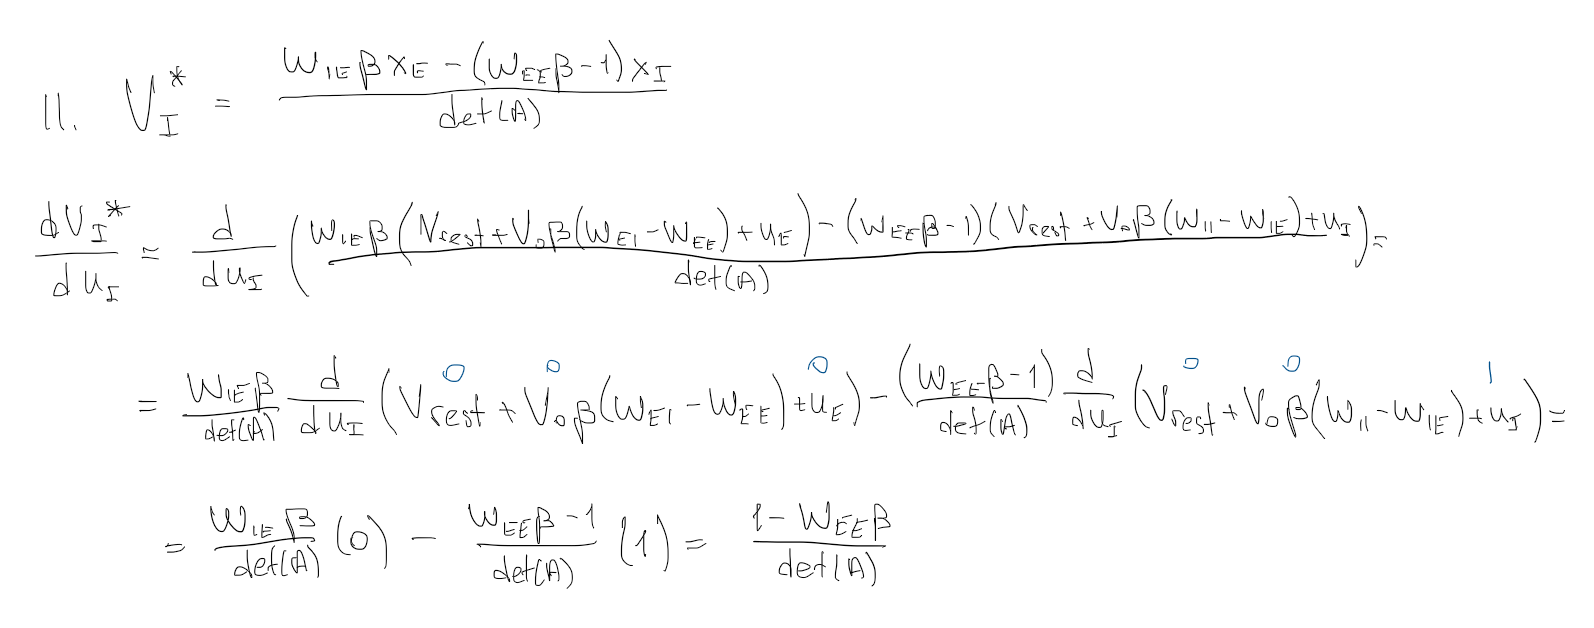
\includegraphics[width=1\textwidth]{images/dvi_derivation.png}
    \label{fig:dvi-derivation}
\end{figure}
% \noindent
\clearpage
\section{Python code for simulations}
% \begin{lstlisting}[style=python,caption=Python code for simulations]
\begin{minted}[mathescape, linenos,]{python}
import numpy as np
import matplotlib.pyplot as plt
import matplotlib 
font = {
        'weight' : 'bold',
        'size'   : 12
}
matplotlib.rc('font', **font)

class EI_Network:
    def __init__(self):
        self.selected_network = 0
        self.V_I_clamp = False
        # neuron params
        self.beta = 1
        self.tau_E = 20
        self.tau_I = 10
        self.V_init = -55
        self.V_rest = -70
        # connection weights
        self.W_EI = 0.65
        self.W_IE = 1.2
        self.W_II = 0.5
        self.W_EE = 0
        # results
        self.VI = np.array([])
        self.VE = np.array([])
        
    def phi(self, V):
        # relu activation function
        v = self.beta * (V - self.V_init)
        return v * (v > 0)
    
    def select_network(self, network_number):
        self.selected_network = network_number
        if network_number == 1:
            self.W_EE = 0.5
        elif network_number == 2:
            # self.W_EE = 1.25
            self.W_EE = 1.25
        elif network_number == 3:
            # isolated excitatory network
            self.W_EE = 1
            self.W_EI = 0.0
            self.W_IE = 0.0
            self.W_II = 1
    
    def set_V_I_clamp(self, V_I_clamp):
        self.V_I_clamp = V_I_clamp

    def euler_simulate(self, N_t, dt, u_e, u_i):
        # figure out how many neurons we are simulating
        u_e_size = len(u_e) if isinstance(u_e, list) else 1
        u_i_size = len(u_i) if isinstance(u_i, list) else 1
        n_neurons = max(u_e_size, u_i_size)
        
        # N_t+1 rows (N_t+init), n_neurons columns
        # Column is V of a SPECIFIC neuron OVER time
        # Row is V for ALL neurons AT a particular time
        VI = np.zeros([N_t+1, n_neurons]) + self.V_rest
        VE = np.zeros([N_t+1, n_neurons]) + self.V_rest
        print(f"Simulating with V_I clamp on: {self.V_I_clamp}")
        for t in range(1, N_t+1):
            ve = VE[t-1]
            vi = VI[t-1]
            # excitatory
            # dVE = -(ve - self.V_rest) + u_e[t]
            dVE = -(ve - self.V_rest)  + self.W_EE * self.phi(ve) - self.W_EI * self.phi(vi) + u_e[t]
            VE[t] = ve + dt * dVE / self.tau_E
            # inhibitory
            # dVI = -(vi - self.V_rest) + u_i[t]
            dVI = -(vi - self.V_rest) + self.W_IE * self.phi(ve) - self.W_II * self.phi(vi) + u_i[t]
            VI[t] = VI[t-1] if self.V_I_clamp else (vi + dt * dVI / self.tau_I) 

        self.VI = VI
        self.VE = VE
    
    def plot_V_and_Phi(self, title):
        # plot Vs and Phi(Vs)
        fig, axs = plt.subplots(1, 2, figsize=(12, 5))
        title = title if title else f'EI Network {self.selected_network}'
        fig.suptitle(title, fontsize=16)
        colors = ['blue', 'red', 'blue', 'red'][::-1]
        linestype = "--" if self.selected_network == 2 else "-"
        # V's
        axs[0].plot(self.VE, label='$V_E$', color=colors[0], linestyle=linestype)
        axs[0].plot(self.VI, label='$V_I$', color=colors[1], linestyle=linestype)
        axs[0].set_xlabel('Time (ms)')
        axs[0].set_ylabel('Voltage (mV)')
        if self.V_I_clamp:
            axs[0].set_ylim(*[-70, 20])
        axs[0].legend()
        axs[0].grid()
        axs[0].set_title('V vs Time')
        # Phi's
        axs[1].plot(self.phi(self.VE), label='$\phi(V_E)$', color=colors[0], linestyle=linestype)
        axs[1].plot(self.phi(self.VI), label='$\phi(V_I)$', color=colors[1], linestyle=linestype)
        axs[1].set_xlabel('Time (ms)')
        axs[1].set_ylabel('$\phi(V)$ $\delta$(mV)')
        if self.V_I_clamp:
            axs[0].set_ylim(*[0, 60])
        axs[1].legend()
        axs[1].grid()
        axs[1].set_title('$\phi(V)$ vs Time')
        # 
        fig.tight_layout(pad=1.0)
        plt.show()

        def plot_2_networks(u_e, u_i, title='EI Network 1 vs 2', V_I_clamp=False):
        """
        Given external input and clamp settings, simulate and plot 2 networks side by side
        """
        colors = ['blue', 'red', 'blue', 'red'][::-1]
        # network 1
        network = EI_Network()
        network.set_V_I_clamp(V_I_clamp)
        network.select_network(1)
        network.euler_simulate(len(u_e)-1, 1, u_e, u_i)
        VE1 = network.VE
        VI1 = network.VI
        # network 2
        network.select_network(2)
        network.euler_simulate(len(u_e)-1, 1, u_e, u_i)
        VE2 = network.VE
        VI2 = network.VI
        # plot
        fig, axs = plt.subplots(1, 2, figsize=(12,5))
        fig.suptitle(title, fontsize=16)
        # V's
        axs[0].plot(VE1, label='$V_E$ (1)', color=colors[0])
        axs[0].plot(VI1, label='$V_I$ (1)', color=colors[1])
        axs[0].plot(VE2, label='$V_E$ (2)', linestyle='--', color=colors[2])
        axs[0].plot(VI2, label='$V_I$ (2)', linestyle='--', color=colors[3])
        axs[0].set_xlabel('Time (ms)')
        axs[0].set_ylabel('Voltage (mV)')
        # limit y axis for clamped V_I
        if V_I_clamp:
            axs[0].set_ylim(*[-70, 20])
        # axs[0].set_ylim(*y_limits)
        axs[0].legend()
        axs[0].grid()
        axs[0].set_title('V vs Time')
        # Phi's
        axs[1].plot(network.phi(VE1), label='$\phi(V_E)$ (1)', color=colors[0])
        axs[1].plot(network.phi(VI1), label='$\phi(V_I)$ (1)', color=colors[1])
        axs[1].plot(network.phi(VE2), label='$\phi(V_E)$ (2)', linestyle='--', color=colors[2])
        axs[1].plot(network.phi(VI2), label='$\phi(V_I)$ (2)', linestyle='--', color=colors[3])
        axs[1].set_xlabel('Time (ms)')
        axs[1].set_ylabel('$\phi(V)$ $\delta$(mV)')
        # limit y axis for clamped V_I
        if V_I_clamp:
            axs[1].set_ylim(*[0, 60])
        axs[1].legend()
        axs[1].grid()
        axs[1].set_title('$\phi(V)$ vs Time')
        # 
        fig.tight_layout(pad=1.0)
        plt.show()

# NO INPUT 
# instantiate the network
network = EI_Network()
# select network 1
network.select_network(1)
# simulate the network
N_t = 300
dt = 0.1
u_e = np.zeros(N_t+1)
u_i = np.zeros(N_t+1)
# plot both networks
plot_2_networks(u_e, u_i, "Networks 1 and 2\n $u_E = u_I = 0$")

# 2. STABLE INPUT
# network 1
# setup
network.select_network(1)
Nt = 500
dt = 1
u_E = np.zeros([Nt+1]) + 20
u_I = np.zeros([Nt+1]) + 20
# simulate
# plot_2_networks(u_E, u_I, "Networks 1 and 2 with $u_E = u_I = 20$")
network.euler_simulate(Nt, dt, u_E, u_I)
network.plot_V_and_Phi("Network 1\n $u_E = u_I = 20$")
# network 2
# setup
network.select_network(2)
Nt = 500
dt = 1
u_E = np.zeros([Nt+1]) + 20
u_I = np.zeros([Nt+1]) + 20
# simulate
network.euler_simulate(Nt, dt, u_E, u_I)
network.plot_V_and_Phi("Network 2\n $u_E = u_I = 20$")
# network 1+2
# for contrast 
u_E = np.zeros([Nt+1]) + 20
u_I = np.zeros([Nt+1]) + 20
plot_2_networks(u_E, u_I, "Networks 1 and 2\n $u_E = u_I = 20$")


# 3. INCREASE INHIBITORY INPUT
# network 1
# setup
Nt = 1000
dt = 1
u_E = np.zeros([Nt+1]) + 20
u_I = np.zeros([Nt+1]) + 20
u_I[500:] = 26
network.select_network(1)
# simulate
network.euler_simulate(Nt, dt, u_E, u_I)
# plot Vs and Phi(Vs)
network.plot_V_and_Phi("Network 1\n $u_E = 20$, $u_{I(:500)} = 20$, $u_{I (500:)} = 26$")
# 4. Network 2
network.select_network(2)
# setup
Nt = 1000
dt = 1
u_E = np.zeros([Nt+1]) + 20
u_I = np.zeros([Nt+1]) + 20
u_I[500:] = 26
# simulate
network.euler_simulate(Nt, dt, u_E, u_I)
# plot Vs and Phi(Vs)
network.plot_V_and_Phi("Network 2\n $u_E = 20$, $u_{I(:500)} = 20$, $u_{I(500:)} = 26$")
# Both networks
# now for contrast, plot both networks together
u_E = np.zeros([Nt+1]) + 20
u_I = np.zeros([Nt+1]) + 20
u_I[500:] = 26
plot_2_networks(u_E, u_I, "Networks 1 and 2\n $u_E = 20$, $u_{I(:500)} = 20$, $u_{I(500:)} = 26$")

# 5. INCREASE EXCITATORY INPUT
# V_I unclamped
# setup
Nt = 1000
dt = 1
u_E = np.zeros([Nt+1]) + 20
u_E[500:] = 26
u_I = np.zeros([Nt+1]) + 20
# simulate unclamped
network.V_I_clamp = False
plot_2_networks(u_E, u_I, "Networks 1 and 2.\n $V_I$ unclamped\n $u_{E(:500)} = 20$, $u_{E(500:)} = 26$, $u_I = 20$")
# V_I clamped
# setup
Nt = 1000
dt = 1
u_E = np.zeros([Nt+1]) + 20
u_E[500:] = 26
u_I = np.zeros([Nt+1]) + 20
# simulate clamped
plot_2_networks(u_E, u_I, "Networks 1 and 2.\n $V_I$ clamped\n $u_{E(:500)} = 20$, $u_{E(500:)} = 26$, $u_I = 20$", V_I_clamp=True)

# Clamped Unclamped Vs on the same graph
# Combining the 2 voltage/time graphs into 1
# simulate and save data
Nt = 1000
dt = 1
u_E = np.zeros([Nt+1]) + 20
u_E[500:] = 26
u_I = np.zeros([Nt+1]) + 20
# setup
network = EI_Network()
# unclamped
network.V_I_clamp = False
network.select_network(1)
network.euler_simulate(Nt, dt, u_E, u_I)
VE1u = network.VE
VI1u = network.VI
network.select_network(2)
network.euler_simulate(Nt, dt, u_E, u_I)
VE2u = network.VE
VI2u = network.VI
# clamped
network.V_I_clamp = True
network.select_network(1)
network.euler_simulate(Nt, dt, u_E, u_I)
VE1c = network.VE
VI1c = network.VI
network.select_network(2)
network.euler_simulate(Nt, dt, u_E, u_I)
VE2c = network.VE
VI2c = network.VI

# plot
colors = ['blue', 'red', 'blue', 'red'][::-1]
title = "Networks 1 and 2.\n $u_{E(:500)} = 20$, $u_{E(500:)} = 26$, $u_I = 20$"

fig, axs = plt.subplots(1, 2, figsize=(12,5))
fig.suptitle(title, fontsize=16)
# V's
axs[0].plot(VE1u, label='$V_E$ (1)', color=colors[0])
axs[0].plot(VI1u, label='$V_I$ (1)', color=colors[1])
axs[0].plot(VE2u, label='$V_E$ (2)', linestyle='--', color=colors[2])
axs[0].plot(VI2u, label='$V_I$ (2)', linestyle='--', color=colors[3])
axs[0].set_xlabel('Time (ms)')
axs[0].set_ylabel('Voltage (mV)')
axs[0].set_ylim([-70, -20])
axs[0].legend()
axs[0].grid()
axs[0].set_title('$V$ vs Time\n$V_I$ unclapmed')
# Phi's
axs[1].plot(VE1c, label='$V_E$ (1)', color=colors[0])
axs[1].plot(VI1c, label='$V_I$ (1)', color=colors[1])
# axs[1].plot(VI1c, label='$V_I$ (1)', color=colors[1])
axs[1].plot(VE2c, label='$V_E$ (2)', linestyle='--', color=colors[2])
axs[1].plot(VI2c, label='$V_I$ (2)', linestyle='--', color=colors[3])
# axs[1].plot(VI2c, label='$V_I$ (2)', linestyle='--', color=colors[3])
axs[1].set_xlabel('Time (ms)')
axs[1].set_ylabel('Voltage (mV)')
axs[1].set_ylim([-70, -20])
axs[1].legend()
axs[1].grid()
axs[1].set_title('$V$ vs Time\n$V_I$ clapmed')
# 
fig.tight_layout(pad=1.0)
plt.show()

\end{minted}

\end{document}
